\subsection{Thermodynamic Theory}
\label{ssec:theory}
    The disordered Ising model will be examined as a \emph{canonical system} in
    \emph{equilibrium}. A canonical system can exchange energy with a
    heat bath, thus has a constant temperature -- the temperature of the
    heat bath.
    Equilibrium is defined as a steady state, where
    the observables are only fluctuating but not changing in any
    particular direction. For example thermal equilibrium denotes the
    condition, that the system under scrutiny has reached the temperature
    of the heat bath. This is the case, once there is no directed energy
    exchange between them, thus the energy of the simulated system reaches
    a steady state, where only fluctuations occur.
    In a canonical ensemble the probability \(p_i\) of a state
    \(i\) is distributed according to a Boltzman distribution
    \begin{equation}
        p_i \propto e^{-\beta H_i}
    \end{equation}
    \begin{equation}
        \beta = \frac{1}{k_B T}
    \end{equation}
    Further the free energy \(F\) of a canonical ensemble is minimized
    in equilibrium and all observables can be derived from \(F\)
    in a straight forward way, as stated in every textbook about
    statistical physics (e.g.\ \cite{nolting2005}).\\
    Because of
    \begin{equation}
        F = U - TS
    \end{equation}
    where \(S\) is the entropy, \(U=\avg{H}\) the internal energy and
    \(\avg{\cdot}\) declares the expected value of an observable.
    One can guess that for low \(T\) the internal energy
    will be low, and for high \(T\) the entropy will be high, to minimize
    \(F\).
    Considering the Hamiltonian of the Ising model, a spin configuration
    of high order, where most spins are aligned with their neighbors,
    leads to a low \(H\) and therefore a low \(U\). Simultaneously, this
    state of high order corresponds to a low entropy \(S\).
    Analogically a state of high \(U\) is also a state of high \(S\).
    These preliminary considerations make a phase transition at some
    \(T\), where the influence of the entropy on \(F\) becomes the same
    order of magnitude as the influence of the internal energy on \(F\),
    very plausible.\\
    To determine
    \begin{equation}
        F=-k_{B}T \ln{Z}
    \end{equation}
    or any expected value of an observable
    \begin{equation}
        \avg{O} = \frac{1}{Z} \sum_i O_i e^{-\beta H_i},
    \end{equation}
    one has to know the partition function
    \begin{equation}
        Z = \sum_i p_i = \sum_i e^{-\beta H_i},
        \label{eq:partitionFunction}
    \end{equation}
    where the sum goes over all possible states \(i\) of the system.
    Because every site can have two states, there are \(2^N\) different
    states of the system. For each the energy \(H_i\) has to be calculated
    to solve the sum from Eq.\ \eqref{eq:partitionFunction} to gain \(Z\).
    Hence for small \(N\) the partition function is computable, but the system
    may show very different properties than in the thermodynamic limit.
    To minimize these finite size effects, it is desirable to examine
    systems with large \(N\). But \(2^N\) is a very rapidly increasing
    number, so for large \(N\) it is unfeasible to calculate the energy for each state, except
    for cases, where it is possible to solve it analytically.\\
    If not, one can get estimates of the observables for big \(N\) using
    Monte Carlo simulations, which are introduced in the next chapter.\\

    The observables which are measured in this thesis are the mean
    magnetization per spin
    \begin{equation}
        m = \frac{1}{N} \sum_i s_i
    \end{equation}
    and the mean energy per spin
    \begin{equation}
        E = \frac{1}{N} \avg{H}.
    \end{equation}
    As mentioned before, properties near the phase transition and the
    critical temperature \(T_c\), where the phase transition occurs, will
    be examined. The Ising system in two dimensions shows a second order
    phase transition, hence \(m\) and \(E\) are continous, but show at
    \(T_c\) an infinitly sharp slope in the thermodynamic limit i.e.\
    the first derivative diverges.
    From statistical physics (compare \cite{nolting2005}) is known that
    these derivatives can be expressed by fluctuations e.g.\ the specific
    heat can be expressed as
    \begin{equation}
        c = \frac{\partial \avg{H}}{\partial T} = k_B \beta^2 \avg{\brac{H-\avg{H}}^2}
    \end{equation}
    The specific heat is a measure for how much energy is needed to change
    the temperature of the system.
    Analogically the susceptibility
    \begin{equation}
        \chi = N \beta \avg{\brac{m-\avg{m}}^2}
    \end{equation}
    is a measure for how strong an outer magnetic field changes the
    magnetization of the system.
    Beside these observables from classical physics, a fifth observable
    the binder cumulant \cite{Binder1981}
    \begin{equation}
        g = \frac{3}{2}\brac{1-\frac{\avg{m^4}}{3\avg{m^2}^2}}
        \label{eq:binder}
    \end{equation}
    is considered.
    This is a dimensionless value, which can be used to determine the
    critical point. These five observables will be sufficient to analyse
    the phase transition in the scope of this bachelor thesis. All of them
    can be easily computed when \(m\) and \(E\) are measured. The next
    chapter will show, how to get estimates for them through Monte Carlo
    simulations.

\subsection{Monte Carlo Simulations}
\label{ssec:montecarlo}
    The idea behind Monte Carlo simulations is to take random samples of
    the observable, which should be measured, and estimate the mean of
    the observable from this samples. To apply this technique to statistical
    ensembles, one creates sample states of the system, measures the
    observables calculates the expected value through averaging.\\
    In statistical physics the expected value of an observable \(O\)
    is -- as also noted above -- calculated by
    \begin{equation}
        \avg{O} = \frac{1}{Z} \sum_i p_i O_i
    \end{equation}
    It is however possible, that there are few states that contribute
    massively more than others. In canonical systems at low \(T\),
    states with low values of \(H\) contribute much more than states with
    high values of \(H\).
    But if one samples the \(2^N\) states evenly, it is probable to miss
    them. this is called \emph{simple sampling} and results in large
    errorbars for any observable.
    It is therefore desirable to sample only the states with high
    contributions to the sum.
    As noted before the system under scrutiny is canonical and therefore
    \(p_i\) is known. The states are distributed according to the Boltzmann
    distribution. Hence \emph{Importance Sampling} can be utilized.\\
    Instead of sampling uniformly distributed random states, one should sample
    states, according to their occurence probability given by the Boltzmann
    distribution. In fact this reduces the estimator to
    \begin{equation}
        O_M = \frac{1}{M} \sum_{i=0}^M O_i,
    \end{equation}
    where \(M\) is the number of samples, as shown in \cite{NewmanBarkema1999}.
    This is a very convenient form.\\
    But it is difficult to create a random state of a physical system,
    e.g.\ the Ising system, according to a given distribution. The simple
    approach of creating uniformly distributed random states and reject
    them with probability \(p_i^{-1}\) depending on their energy is not
    efficient, because many generated states will be discarded and the
    computing time to generate them and caluculating their energy will
    be wasted.
    Hence one uses \emph{Markov Chains} to generate new states \(\nu\)
    from old ones \(\mu\). It is important that the transition probabilities
    \(A(\mu \to \nu)\) obey \emph{Detailed Balance} and \emph{Ergodicity}.
    \emph{Detailed Balance} means that the probability to leave a state is
    the same as the probability to enter the state in equilibrium
    \(p_\mu A(\mu \to \nu) = p_\nu A(\nu \to \mu)\) with \(p_\mu\) the
    probability to be in state \(\mu\). This ensures that the system can
    equilibrate and that the states are distributed according to the
    desired distribution in equilibrium \cite{NewmanBarkema1999}.
    And \emph{Ergodicity} requires that every possible state is reachable
    from every other state in finite time \cite{NewmanBarkema1999} \cite{Katzgraber2011}.
    Otherwise the samples might not be representative for the whole system.\\
    In this thesis three algorithms, which fulfill all requirements,
    were used. They will be shortly described in the following subsections.

    \subsubsection{Metropolis}
        A Metropolis Monte Carlo \cite{Metropolis1953} simulation of an
        Ising model will choose a random spin, calculate the energy change
        \begin{equation}
            \Delta H = H(\nu) - H(\mu)\\
            \label{eq:dH}
        \end{equation}
        that would result from a flip of that spin and execute the flip
        with the probability \cite{NewmanBarkema1999} \cite{Katzgraber2011}
        \begin{equation}
            A(\mu \to \nu) =
            \begin{cases}
                1                            & \Delta H \le 0 \\
                \exp{\brac{-\beta \Delta H}} & \Delta H > 0
            \end{cases}.
            \label{eq:metropolis}
        \end{equation}
        So if a transition lowers the energy it will be always done. This
        results in a high ratio between chosen spins and flipped spins.
        Therefore it minimizes the calculations needed for a change of
        the state. Also note that \(\Delta H\) is easy to calculate,
        because it is only affected by the spin of the neighbors of the
        chosen site.

    \subsubsection{Wolff}
    \label{sssec:wolff}
        Close to the critical temperature \(T_c\) the Metropolis
        gets slower. This is called \emph{critical slowing} down.\\
        In order to circumvent this a cluster algorithm like the Wolff
        algorithm \cite{Wolff1989} can be used.
        For an Ising model the Wolff algorithm builds a cluster of sites
        starting with a random site and adding neighboring sites of the
        same spin with probability
        \begin{equation}
            P_{\mathrm{add}} = 1-\exp\brac{-2\beta J},
            \label{eq:wolffAdd}
        \end{equation}
        where \(J\) is the coupling constant (c.f.\ Sec.\ \ref{ssec:isingmodel}).
        The neighboring sites of the added sites
        are also considered and so forth. When there are no more sites
        to add, the spin of every site in the cluster is flipped
        \cite[p. 91ff]{NewmanBarkema1999} \cite[p. 151f]{Katzgraber2011}.
        This leads fast to new uncorrelated states at the critical
        temperature because big clusters are flipped. But there are not
        much advantages at high or low temperatures. At low temperatures
        the cluster will consist of almost all sites such that all but
        very few spins will be flipped. At high temperatures the cluster
        will only contain very few sites.
        Both situations have no advantage against the Metropolis algorithm.\\
        So one would activate this algorithm near the critical temperature
        but would use a simple Metropolis algorithm at high and low temperatures.

    \subsubsection{Parallel Tempering}
        In simulations using \emph{parallel tempering} \cite{ParallelTempering1986}
        many identical systems at different temperatures are simulated and
        the spin configurations between two neighboring temperatures are
        swapped periodically with probability \cite[p. 169ff]{NewmanBarkema1999} \cite[S. 155ff]{Katzgraber2011}
        \begin{equation}
            P((E_i,T_i) \to (E_{i+1},T_{i+1})) = \min\brac{1,\exp\brac{\brac{E_{i+1}-E_i}\brac{\frac{1}{T_{i+1}}-\frac{1}{T_i}}}},
            \label{eq:partemp}
        \end{equation}
        as schematically pictured in Fig.\ \ref{fig:parTemp}\subref{sfig:parTemp:schema}.
        This has the advantage that correlation times of single
        temperatures are far smaller, because their spin configuration
        gets often replaced by another uncorrelated configuration. In
        many cases the more important advantage is that a system which
        is trapped in a local minimum at a given temperature can travel
        to higher temperatures, leave its local minimum and cool down
        again in a lower minimum. If a system is trapped in such a
        metastable state, ergodicity is not guaranteed anymore.
        This is schematically pictured in Fig.\ \ref{fig:parTemp}\subref{sfig:parTemp:E}.
        \begin{figure}[htbp]
            \centering
            \subfigure[Schematic Diagramm of the Algorithm][]{
                \label{sfig:parTemp:schema}
                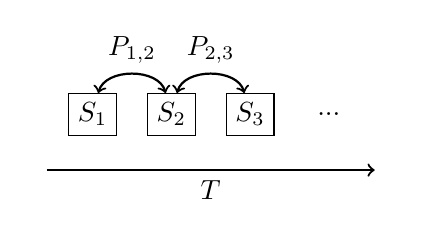
\begin{tikzpicture}
    \node[draw,rectangle] (a) {$S_1$};
    \node[draw,rectangle,right of=a] (b) {$S_2$};
    \node[draw,rectangle,right of=b] (c) {$S_3$};
    \node[rectangle,right of=c] (d) {...};

    \node[rectangle,below left of=a] (A) {};
    \node[rectangle,below right of=d] (D) {};
    \draw[thick,->] (A) edge node[below] {$T$} (D);

    \draw[thick,<->] (a) edge[out=75,in=105] node[above] {$P_{1,2}$} (b);
    \draw[thick,<->] (b) edge[out=75,in=105] node[above] {$P_{2,3}$} (c);
    %~ \draw[thick,<->] (c) edge[out=80,in=100] node[above] {$P_{..}$} (d);
\end{tikzpicture}

            }
            \subfigure[Schematic Diagramm of the Energy Landscape][]{
                \label{sfig:parTemp:E}
                \documentclass{standalone}
\usepackage{tikz}

\begin{document}
    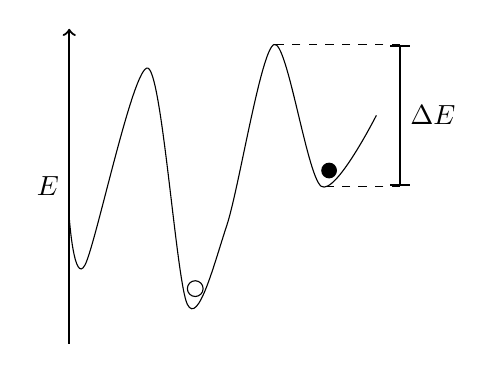
\begin{tikzpicture}
        %~ \draw[thick,->] (0,0) -- node[below] {$T$} (6,0);
        \draw[thick,->] (0,0) -- node[left] {$E$} (0,4);

        \draw plot [smooth] coordinates {(0,1.6) (0.2,1) (1,3.5) (1.5,0.5) (2,1.5) (2.6,3.8) (3.2,2) (3.9,2.9)};

        \fill (3.3,2.2) circle(0.1);
        \draw (1.6,0.7) circle(0.1);

        \draw[thick,|-|] (4.2,2) -- node[right] {$\Delta E$} (4.2,3.8);
        \draw[dashed] (4.2,2) -- (3.2,2);
        \draw[dashed] (4.2,3.8) -- (2.6,3.8);
    \end{tikzpicture}
\end{document}

            }
            \caption[Visualisation of the Parallel Tempering Algorithm]
            {
                \subref{sfig:parTemp:schema} schematic representation of
                the swapping of spin configurations of different simulations \(S_i\)
                between temperatures.\\
                \subref{sfig:parTemp:E} sketch of an energy landscape, where
                the state of the system (filled dot) is trapped in an local
                minimum. At low temperatures it is very unlikley that it
                overcomes the energy barrier \(\Delta E\) to the minimum.
                After a swap to higher energies, the barrier can be overcome
                and after a swap to lower energies again, the state in
                the minimum can be reached (hollow dot).
            }
            \label{fig:parTemp}
        \end{figure}\\
        In the case of a ferromagnetic Ising model the risk to get trapped
        in an local energy minimum is very low. Consequently the autocorrelation
        decreases significantly. In the scope of this thesis this comes
        for no cost, because one has to simulate for many temperatures
        to determine the critical temperature. The additional calculations
        to determine whether to swap configurations or not are small in
        comparison with those that would be needed to generate a new
        uncorrelated state without \emph{parallel tempering}.

    \subsubsection{Implementation Details}
        Here a mixture of the above three algorithms is used.
        For each sweep \(N\) Metropolis spin flips, one Wolff cluster flip
        and one parallel tempering swap are performed. Where \(N\) is the
        number of sites.\\
        Because it is not known before, where the critical temperatures
        \(T_c\) are located, the Wolff cluster algorithm is used for
        every temperature. The speed up near criticality is worth the
        moderate slow down at other temperatures.

    \subsubsection{Equilibration- and Autocorrelation Time}
    \label{sssec:eqtime}
        To generate states acoording to the Boltzmann distribution at a
        given temperature \(T\), one starts with an arbitrary state
        and waits until it reaches thermal \emph{equilibrium}. Because
        equilibrium is defined as a steady state, one can determine it by
        observing the change of the observables over the progressing
        simulation, as pictured in Fig.\ \ref{fig:equiandauto}\subref{sfig:equiandauto:equiE}.
        The count of sweeps till
        equilibrium is called \emph{equilibration time} \(t_{eq}\).
        All measurements should start after this time.\\
        In Fig.\ \ref{fig:equiandauto}\subref{sfig:equiandauto:equiE}
        the equilibrium is reached after approximately \(N_{s} \approx 50\) sweeps for
        both an initial condition of all spins up and all spins random. It
        does not harm to double that value to be save. Particularly, because
        it is a random process, so that there can not be an exact value.
        \begin{figure}[htbp]
            \centering
            \subfigure[Example of an Equilibrating Ising System][]{
                    \label{sfig:equiandauto:equiE}
                    \includegraphics[width=0.47\textwidth]{plots/equiE}
            }
            \subfigure[Example of the Autocorrelation of an Ising System][]{
                    \label{sfig:equiandauto:autoM}
                    \includegraphics[width=0.47\textwidth]{plots/autoM}
            }
            \caption[Examples for Equilibration and Autocorrelation]
            {
                \subref{sfig:equiandauto:equiE} Example of an Ising system
                    \(L=64\) reaching thermal equilibrium at \(T=2.36\) after
                    approximately \(n=50\) sweeps.\\
                \subref{sfig:equiandauto:autoM} The autocorrelation of an
                    Ising system \(L=64\) at \(T=2.40\) (only Metropolis
                    sweeps -- otherwise the decline is too steep to show)
                    on half logarithmic axis.
                    The straight line is an exponential fit \(\exp(-t/\tau)\)
                    with \(\tau = 342(1)\).
            }
            \label{fig:equiandauto}
        \end{figure}\\
        Because every state is generated from the state before, measurements
        of subsequent states are correlated. To determine when two states
        are independent, one calculates the normalized autocorrelation function
        \(\frac{\chi(t)}{\chi(0)}\) with
        \begin{equation}
            \chi(t) = \int \mathrm{d} t' \, [m(t') -\avg{m}][m(t'+t)-\avg{m}],
        \end{equation}
        which decays exponentially
        \(\chi(t) \propto \exp(t/\tau)\). This is visible in the half
        logarithmic plot \ref{fig:equiandauto}\subref{sfig:equiandauto:autoM}.
        To get the autocorrelation time one can either fit a exponential
        function \(\exp(-t/\tau)\) like in Fig.\ \ref{fig:equiandauto}\subref{sfig:equiandauto:autoM}
        or integrate \(\tau = \int \frac{\chi(t)}{\chi(0)} \de t\).
        \(\tau\) is an estimate that specifies the time after which two
        samples are not correlated anymore \cite[p. 59ff]{NewmanBarkema1999} \cite[p. 150f]{Katzgraber2011}.
        To ensure that the error is not underestimated one should wait
        \(2\tau\) sweeps between two measurements.
        The autocorrelation time is dependent on the temperature.
        For example for the standard Metropolis algorithm the fluctuations
        are strong at high temperatures and subsequent
        states are more dissimilar and therefore less correlated than at low
        temperatures, where less spins are flipping. But the longest
        autocorrelation times are encountered at the critical temperature.
        This effect is called \emph{critical slowing down} and is
        characterized by the \emph{dynamical critical exponent} \(z\)
        \cite{SwendsenWang1987}. The dependence of the autocorrelation time
        \(\tau\) on the system size \(L\) is at \(T_{c}\) given by \(\tau \propto L^z\).
        More general the power law \(\tau \propto \xi^z\) holds true, where
        \(\xi\) is the \emph{correlation length}, which diverges at
        \(T_{c}\) and is then limited by the size of the simulated lattice.
        As mentioned in Sec.\ \ref{sssec:wolff}, the Wolff cluster algorithm
        decreases \(z\) dramatically. This causes the course of the autocorrelation
        time in dependence on temperature to change significantly as shown in
        Sec.\ \ref{ssec:results:autocorr}. Also according to \cite{NewmanBarkema1999}
        \(z\) is independent of the lattice structure, which ensures that
        the simulation will benefit from the Wolff cluster algorithm at
        any \(\sigma\).
